% "ККМ"

\documentclass[a4paper,12pt]{article} % тип документа

% article, report, book

%  Русский язык

\usepackage[T2A]{fontenc}			% кодировка
\usepackage[utf8]{inputenc}			% кодировка исходного текста
\usepackage[english,russian]{babel}	% локализация и переносы


% Математика
\usepackage{amsmath,amsfonts,amssymb,amsthm,mathtools} 


\usepackage{wasysym}

%Заговолок


\author{Фролова Светлана \\ Киселев Анатолий}
\title{ОТЧЕТ\\
О ЛАБОРАТОРНОЙ РАБОТЕ\\
по теме:\\
Определение ККМ в растворах ПАВ\\
по измерению электропроводности и\\
поверхностного натяжения
}
\date{МФТИ\\г. Долгопрудный\\[0.5cm]28 февраля 2018 г.}

\begin{document}

\maketitle

\newpage

\section{Цели работы}
\begin{enumerate}

\item Освоение методик определения критической концентрации мицеллообразования
ионогенных и неионогенных ПАВ по измерениям электропроводности и
поверхностного натяжения раствора;
\item оценка степени ионизации мицелл ионогенных ПАВ по результатам
кондуктометрических измерений;
\item построение изотермы поверхностного натяжения и адсорбции ПАВ на поверхности
раствора. Определение площади, занимаемой молекулой ПАВ в насыщенном
адсорбционном слое.
\end{enumerate}

\newpage

\section{Теоретическая часть}
\subsection*{}
ПАВ – химические соединения, которые, концентрируясь на поверхности раздела термодинамических фаз, вызывают снижение поверхностного натяжения. ПАВ делятся на ионогенные и неионогенные. \\
Спонтанное формирование монослойных и бислойных структур молекулами ПАВ: 
Молекулы ПАВ с длинными или крупными углеводородными радикалами обладают особенно выраженными поверхностно-активными свойствами. Известно, что высокое поверхностное натяжение воды обусловлено ее склонностью к образованию водородных связей. Вблизи неполярный фазы или неполярных частиц происходит искажение структуры воды, образованной сетью водородных связей. Соответственно, чем больше поверхность неполярного (олеофильного) объекта, тем менее выгодно его нахождение в воде. Вода стремится уменьшить площадь границы раздела, объединяя такие объекты в ассоциаты или крупные капли.
\subsection*{}
Тип формируемых липидами и другими ПАВ структур определяется их концентрацией и формой молекул. Давно замечено, что существенным является соотношение размеров (ширины) головки и хвоста молекулы. Если головка крупнее хвоста, молекулы липидов стремятся формировать мицеллы или занимать внешнюю сторону липосом или липидных трубок. Такие молекулы зачастую называют «мальчиками». Молекулы, у которых наоборот, хвост крупнее головки (так называемые «девочки»), стремятся собраться на внутренней стороне липосом или формировать обратные мицеллы. Плоские липидные бислои могут образовываться только из липидов с близкими размерами хвоста и головки, либо из смеси «мальчиков» и девочек». 

Критическая концентрация мицеллообразования— концентрация по-верхностно-активного вещества в растворе, при которой образуются устойчивые мицеллы. 
Факторы влияющие на ККМ: 
\begin{enumerate}
\item Влияние УВ радикала на ККМ 
Склонность к мицеллообразованию, как и поверхностная активность, существенно увеличиваются с длиной углеводородного радикала. Для водных растворов – в соответствии с правилом Дюкло-Траубе поверхностная активность соседних членов гомологического ряда различается в 3,2 раза. Способность к ассоциации и мицеллообразованию проявляется у молекул ПАВ при $n > 8 - 10$ атомов углерода С. 
\item Влияние посторонних электролитов на ККМ. 

Введение электролитов в растворы ионогенных и неионогенных ПАВ вызывает различный эффект. В растворах ионогенных ПАВ с ростом концентрации индифферентных электролитов величина ККМ снижается. В этом эффекте можно выделить несколько причин. Основную роль играют концентрация и заряд противоионов, определяющие создаваемую ионную силу раствора. Облегчение мицеллообразования с ростом ионной силы объясняется сжатием диффузной части двойного электрического слоя противоионов и подавлением диссоциации молекул ПАВ. Кроме этого происходит частичная дегидратация заряженных головок ПАВ (конкуренция с ионами добавленного электролита). Все это облегчает сборку заряженных молекул ПАВ в мицеллы. При 
добавлении индифферентного электролита мицеллярная масса ионогенных ПАВ растет, величина ККМ снижается. Мицеллярная масса неионогенных ПАВ и их ККМ практически не изменяется при изменении ионной силы раствора Наконец, противоионы постороннего электролита могут специфически взаимодействовать с заряженными группами ионогенных ПАВ, что также сказывается на величине ККМ. Меньшая гидратация противоионов способствует их меньшему отталкиванию и лучшей адсорбции на поверхности мицелл. В результате этой адсорбции уменьшается заряд мицелл, взаимное отталкивание составляющих их молекул ПАВ, а, следовательно, и величина ККМ. Ионы одинаковой валентности по способности снижать ККМ располагаются в так называемые лиотропные ряды. 
\item Влияние добавки органических веществ. 
\item Влияние температуры.
\end{enumerate}
Исследования водных растворов ионогенных ПАВ показали, что мицеллообразование может происходить только выше некоторой температуры $T_\text{k}$, называемой точкой Крафта. Многие ПАВ с большим углеводородным радикалом из-за плохой растворимости в воде не образуют мицеллярных растворов. Однако при увеличении температуры их растворимость растет и может начаться мицеллообразование. По определению точкой Крафта называется температура, при которой резко увеличивается растворимость ионогенных ПАВ в результате образования мицелл. Ниже этой температуры растворимость ПАВ слишком мала для образования мицелл. Обычно точка Крафта лежит в интервале $10-20^oC $
\subsection*{Методы измерения ККМ}
\subsubsection*{Кондуктометрический метод}
Кондуктометрическое определение ККМ основано на измерении
концентрационной зависимости электропроводности растворов ионогенных ПАВ. Если
бы в водных растворах ионогенных ПАВ, отсутствовало мицеллообразование, то в
согласии с уравнением Кольрауша, экспериментально измеренная эквивалентная
электропроводность в зависимости от квадратного корня из концентрации описывалась
бы линейной функцией. Это выполняется при малых концентрациях ПАВ (менее
$10^{-3}$ М), а начиная с ККМ формируются ионные мицеллы, окруженные диффузным слоем
противоионов, и на экспериментальной зависимости наблюдается излом, обусловленный
образованием сферических ионных мицелл.
Подвижности ионных
мицелл меньше
подвижности ионов.
Кроме того,
значительная часть
противоионов
находится в плотном
адсорбционном слое,
что существенно
уменьшает
электропроводность
раствора ПАВ (заряд
мицелл меньше
суммарного заряда составляющих их молекул ионогенного ПАВ). Поэтому при
увеличении концентрации ПАВ выше ККМ наблюдается уменьшение скорости роста
удельной электропроводности.

\subsubsection*{Метод поверхностного натяжения}
Поверхностное натяжение водных растворов ПАВ уменьшается с ростом
концентрации вплоть до ККМ. Изотерма поверхностного натяжения, $\sigma = f (ln
{c_{\text{пав}}})$ в области низких концентраций ПАВ имеет криволинейный участок, на котором в
соответствии с уравнением адсорбции Гиббса адсорбция Г на межфазной границе
возрастает с ростом концентрации:
\[-d\sigma = RT \cdot \text{Г} \ln{c_{\text{пав}}}\]
При определенной пороговой концентрации сm криволинейный участок изотермы
переходит в линейный участок с постоянным наклоном , т.е. адсорбция
достигает постоянного и максимального значения. В этой области на межфазной границе
формируется насыщенный мономолекулярный
адсорбционный слой. При дальнейшем
увеличении общей концентрации ПАВ ($c_{\text{пав}} >
\text{ККМ}$) концентрация молекулярного раствора
ПАВ перестает расти, в объеме раствора
увеличивается концентрация мицелл, и
поверхностное натяжение остается практически
постоянным. Величина ККМ определяется по
излому изотермы при выходе ее на
горизонтальный участок.

\newpage

\section{Ход работы}
\subsection{Кондуктометрический метод}
Для проведение измерений были приготовлены растворы объемами по 25 мл заданных концентраций ТТАВ (тетрадецилтриметиламмония бромида). Для определения удельной электропроводности приготовленные растворы наливали в кондуктометрическую ячейку.\\
\begin{table}[h!]
\centering
\caption{}
\label{my-label}
\begin{tabular}{|l|l|l|l|l|}
\hline
№  & $C_{\text{пав}}$ & $\sqrt{C_{\text{пав}}}$ & K, $\text{мкСм}\cdot\text{см}^{-1}$ & экв. элект-сть \\
\hline
1  & 0,1    & 0,316        & 15,7                          & 157,000       \\
\hline
2  & 0,5    & 0,707        & 51,9                          & 103,800       \\
\hline
3  & 1,5    & 1,225        & 148,3                         & 98,867        \\
\hline
4  & 3      & 1,732        & 297                           & 99,000        \\
\hline
5  & 5      & 2,236        & 372                           & 74,400        \\
\hline
6  & 6      & 2,449        & 395                           & 65,833        \\
\hline
7  & 8      & 2,828        & 418                           & 52,250        \\
\hline
8  & 12     & 3,464        & 552                           & 46,000        \\
\hline
9  & 15     & 3,873        & 600                           & 40,000        \\
\hline
10 & 18     & 4,243        & 672                           & 37,333        \\
\hline
11 & 20     & 4,472        & 722                           & 36,100        \\
\hline

\end{tabular}
\end{table}\\
По излому графиков определили значение ККМ: 
ККМ = 8 мМ 
Табличное значение ККМ: 6,8 мМ

\newpage

\begin{figure}[t]

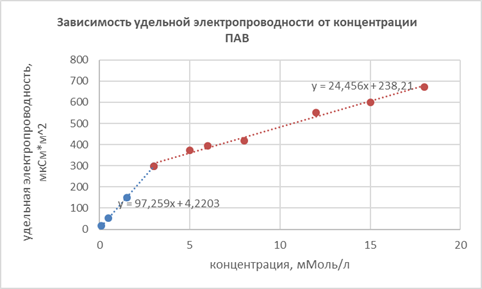
\includegraphics[width=1\textwidth]{image009.png}
\caption{}
\end{figure}

\begin{figure}[h!]
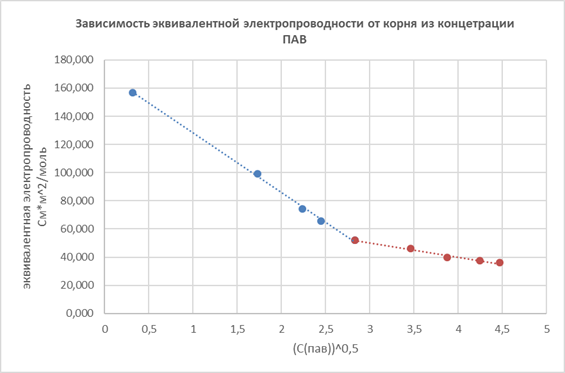
\includegraphics[width=1\textwidth]{image008.png}
\caption{}
\end{figure}


\newpage


\subsection{Метод поверхностного натяжения}

\begin{table}[h!]
\centering
\caption{}
\label{my-label}
\begin{tabular}{|l|l|l|l|l|l|l|}
\hline
$F_{\text{пов},1}/g$ & $F_{\text{пов},2}/g$ & $F_{\text{пов},3}/g$ & $<F_{\text{пов}}>/g$          & $C$   & $\sigma=F/2l$ & $\lg C$      \\
\hline
1503      & 1508      & 1506      & 1505,666667 & 0   & 73,777667  & --       \\
\hline
1387      & 1359      & 1368      & 1371,333333 & 0,1 & 67,195333  & -1       \\
\hline
1421      & 1433      & 1421      & 1425        & 0,2 & 69,825     & -0,69897 \\
\hline
1306      & 1299      & 1301      & 1302        & 0,6 & 63,798     & -0,22185 \\
\hline
1181      & 1186      & 1181      & 1182,666667 & 1   & 57,950667  & 0        \\
\hline
980       & 983       & 979       & 980,6666667 & 2   & 48,052667  & 0,30103  \\
\hline
854       & 850       & 841       & 848,3333333 & 4   & 41,568333  & 0,60206  \\
\hline
819       & 832       & 823       & 824,6666667 & 6   & 40,408667  & 0,778151 \\
\hline
824       & 835       & 830       & 829,6666667 & 8   & 40,653667  & 0,90309  \\
\hline
826       & 829       & 830       & 828,3333333 & 12  & 40,588333  & 1,079181 \\
\hline
815       & 824       & 812       & 817         & 20  & 40,033     & 1,30103  \\
\hline
\end{tabular}
\end{table}

\begin{figure}[h]
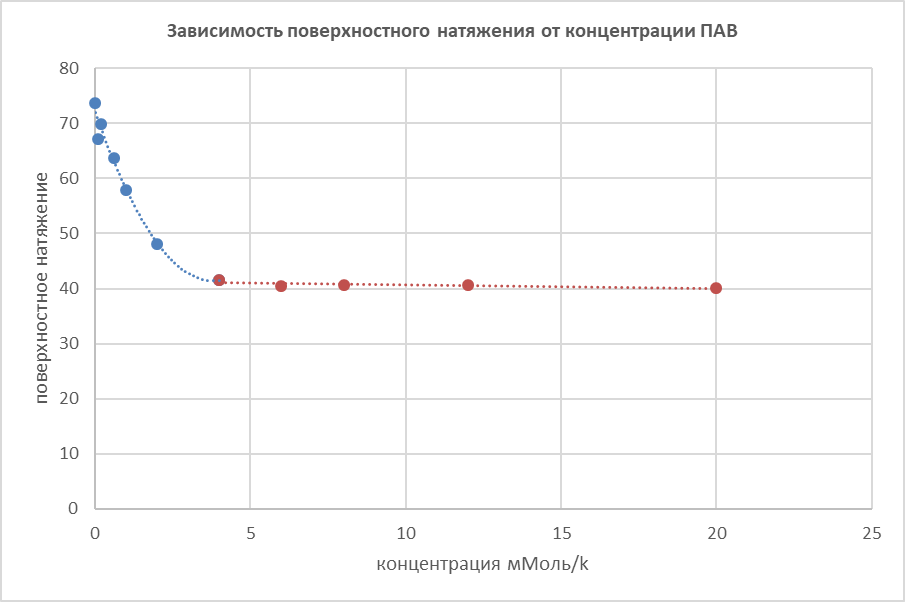
\includegraphics[width=1\textwidth]{image003.png}
\caption{}
\end{figure}

\begin{figure}[h!]
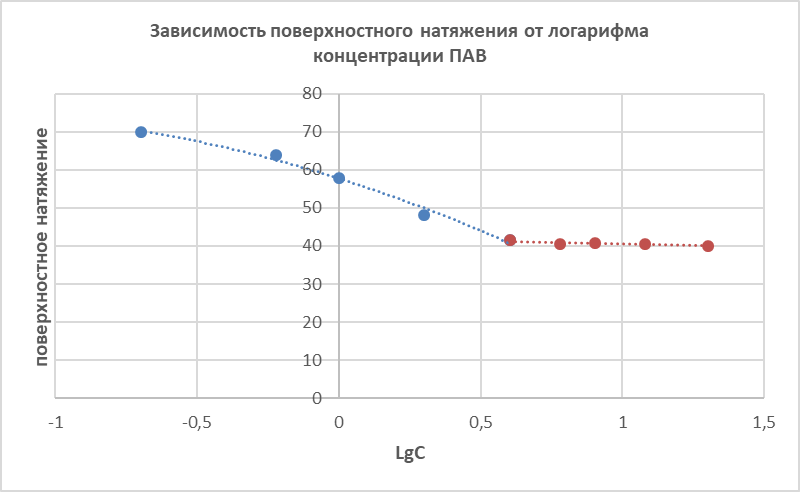
\includegraphics[width=1\textwidth]{image007.png}
\caption{}
\end{figure}
Предельную адсорбцию определили из угла наклона графика зависимости поверхностного натяжения от логарифма концентрации. 
\[\text{Г}_\infty = 9\cdot10^{-6} \text{моль}/\text{м}^2\]
Площадь приходящаяся на одну частицу в плотном монослое на поверхности раствора: 
$S_0 = 1,8457\cdot10^{-19}\text{м}^2$\\
Длина молекулы в плотном слое: $0,0030276\cdot10^{-3}$ м
\newpage
\section{Вывод}
\begin{enumerate}
\item  Определили критическую концентрацию мицелообразования ТТАВ двумя методами: 
Кондуктометрическим и методом поверхностного натяжения. 
\item Определили предельную адсорбцию, площадь занимаемой одной молекулой ПАВ а также ее длину. 
\item Построили изотерму поверхностного натяжения от концентрации и от логарифма концентрации.

\end{enumerate}
\end{document}